\documentclass[crop,tikz,convert={outext=.svg,command=\unexpanded{pdf2svg \infile\space\outfile}},multi=false]{standalone}[2012/04/13]

\usepackage[utf8]{inputenc}
\usepackage{amsmath, amssymb}
\usepackage{pgfplots}
%-------------------------------------
% Tikz and pgf options & definitions
%-------------------------------------
\pgfplotsset{compat=1.15}
\pgfmathsetseed{1}

\usetikzlibrary{positioning}
\usetikzlibrary{shapes}
\usetikzlibrary{backgrounds, fit}
\usetikzlibrary{calc}
\usetikzlibrary{decorations.markings}
\usetikzlibrary{matrix}

\def\colorvector at (#1,#2,#3){
\coordinate (A) at (#1, #2);
\filldraw[draw=black,fill=test!!+] (A)++(0,0) rectangle ++(0.25,0.25) node (A0) {};
\filldraw[draw=black,fill=test!!+] (A)++(0.3,0) rectangle ++(0.25,0.25) node (A1) {};
\filldraw[draw=black,fill=test!!+] (A)++(0.6,0) rectangle ++(0.25,0.25) node (A2) {};
\node[right=of A2, xshift=-7.5ex, yshift=-0.75ex] {$\ldots$};
\filldraw[draw=black,fill=test!!+] (A)++(1.5,0) rectangle ++(0.25,0.25) node (A4) {};
\node[left=of A1, xshift=4.4ex, yshift=-0.75ex] (BEG\i) {$#3=[$};
\node[right=of A4, xshift=-8ex, yshift=-0.75ex] (END\i) {$]^{T}$};
}

\begin{document}
\tikzset{every loop/.style={min distance=15mm,looseness=10}}
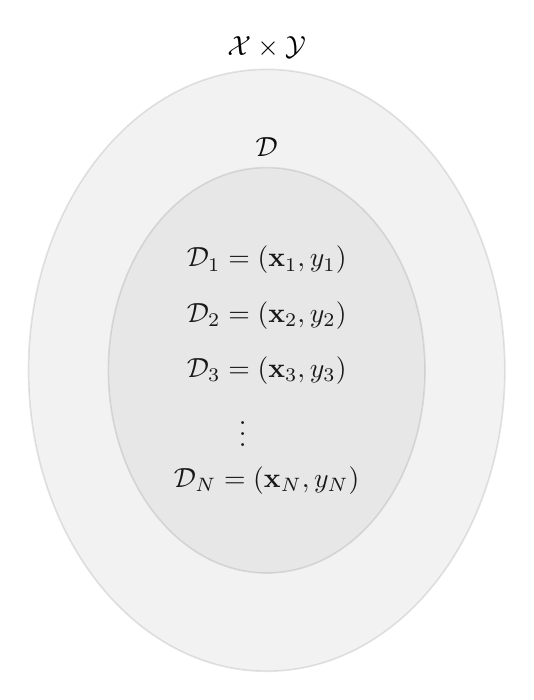
\begin{tikzpicture}[-latex ,auto ,node distance =0.7cm and 5cm, on grid,semithick ,
state/.style ={circle, draw, color=blue , fill=blue, text=white , minimum width =0.2 cm}]
\node[] (D1) {${\cal D}_{1} = \left( {\bf x}_{1}, y_{1} \right) $};
\node[] (D2) [below =of D1]{${\cal D}_{2} = \left( {\bf x}_{2}, y_{2} \right) $};
\node[] (D3) [below =of D2]{${\cal D}_{3} = \left( {\bf x}_{3}, y_{3} \right) $};
\node[] (Ddots) [below =of D3][label=left:$\vdots$]{};
\node[] (DN) [below =of Ddots]{${\cal D}_{N} = \left( {\bf x}_{N}, y_{N} \right) $};
\node[fit={(D1)(DN)},draw, ellipse, fill=gray, opacity = 0.1, minimum width=3cm,minimum height=5cm,label=above:{${\cal D}$}](D){};
\node[fit={(D)},draw, ellipse, fill=gray, opacity = 0.1, minimum width=3cm,minimum height=5cm,label=above:{${\cal X} \times {\cal Y}$}](XY){};
\fill[even odd rule, gray] (XY) (D);
\end{tikzpicture}
\end{document}